
\section{Mac OS}
\begin{figure}[H]
    \centering
    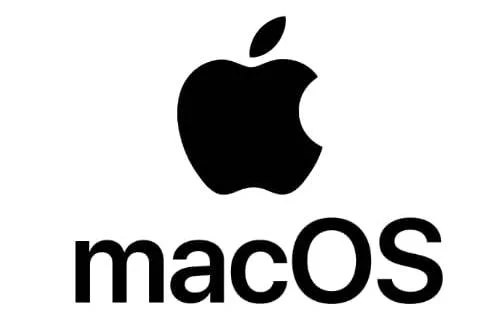
\includegraphics[width=0.3\textwidth]{figures/macOS.png}
    \caption[Ícono de macOS]%
            {Ícono de macOS \citep{GQInfo_macOS}}
    \label{fig:sistema_operativo_mac_os}
\end{figure}
El proyecto Mach dio comienzo en 1985 en la universidad de Carnegie Mellon con la finalidad de crear un microkernel que reemplace al BSD. Su diseño buscaba más seguridad para los usuarios, nose genero lo resultados esperados y se cancelo en 1994. Entonces el proyecto fue adoptado pro OSF/1 Y NeXTSTEP por lo que completo al combinar los componente de BSD, dando origen al kernel XNU de tipo monolítico, pero presento limitaciones con el System 7 y fracaso el proyecto, por ultimo este último avance fue adquirida por Steve Jobs, lo que permitió integrar NeXTSTEP y su kernel XNU como nuevo sistema operativo a Mac OS X, lanzado en 24 marzo del 2001 con el kernel de XNU, que integraba Mach 3.0 y el marco I/O kit, además de ser integrado en Intel Y ARM \citep{Keuper2012}.
El kernel de XNU prosee una arquitectura hibrida que tiene 4 componentes clave \textbf{Mach} que se encarga de administrar las tares, que contine hilos. Su caracteristica principal es la mensajería, mediante puntos de comunicación (IPC), usa el Mach Interface Generator (MIG) para acortar lo procesos, tenemos tambien \textbf{BDS} que implementa procesos y señales UNIX, adema de sistema de archivos y redes, \textbf{I/O Kit} es el marco de controladores orientado a objetos y por ultimo \textbf{KEXTs}  que encargar de enlazar  no solo con el I/O Kit, sino tambien con otras partes del kernel, extensión de red, sistema de archivos \citep{Levin2007}.
Varios de los primeros trabajos de software abierto de Apple son Darwin y WebKit. Darwin es un sistema operativo público que Apple introdujo en el año 2000. Este sistema fue liberado bajo la Licencia Pública de Apple (APSL), que ha sido aceptada por la OSI y la FSF \citep{Levin2007}